%!TEX root = ../main.tex
\chapter{Methods}
Reverse engineering is a complex process with no universal solution. It often involves extensive trial and error, making it important to adopt a strategy that encourages rapid iteration while minimizing risk. In this case, the most practical approach was to prioritize simplicity and accessibility. The Android version of the app was selected for analysis, as it uses Java and Kotlin—languages that are generally more amenable to reverse engineering. Additionally, a man-in-the-middle (MITM) technique was chosen to intercept and manipulate data exchanged between the app and the target device.

The initial step involved verifying the ability to interact with the app by modifying data in a detectable way. Once this was confirmed, the next objective was to capture the data being transmitted between the app and the makeup printing device, along with identifying the method of transmission. The final step was to replicate that communication in order to send custom data to the device in the expected format.

Java is particularly well-suited for reverse engineering due to its architecture. It is designed to be platform-independent by running on the Java Virtual Machine (JVM), which functions as an abstract computing environment with its own instruction set and memory model. The JVM interprets a binary format known as a class file, which contains bytecode (JVM instructions), a symbol table, and metadata.

The JVM is stack-oriented, with most operations involving the operand stack in the current execution frame. New frames are created whenever methods are invoked, providing a clear and modular structure. This design simplifies the decompilation and analysis process, which is critical when reconstructing application logic and behavior (Oracle JVM Specification, SE8).
Figure [insert number] illustrates the flow of data from Java source code through compilation, class loading, bytecode verification, and execution by the JVM.
\begin{figure}
	\centering
	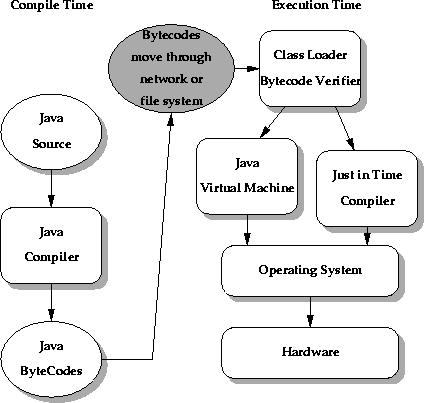
\includegraphics[width=0.7\linewidth]{java_process}
	\caption{}
	\label{fig:javaprocess}
\end{figure}

The use of class files is one of the key factors that makes reverse engineering Java-based applications more straightforward. Unlike many other languages that are compiled directly into low-level assembly, Java is compiled into bytecode, an intermediate representation that retains a significant amount of the original structure of the source code. This structure provides helpful context for decompilation tools.
As noted in Covert Java™: Techniques for Decompiling, Patching, and Reverse Engineering by Alex Kalinovsky, “bytecode can be interpreted or compiled after loading, which results in a two-step transformation of the high-level programming language into the low-level machine code. It is the intermediate step that makes decompiling Java bytecode nearly flawless” (javaRE). Bytecode preserves nearly all critical information from the source file, with the exception of comments and formatting. Method names, variables, and control flow are typically intact, making it easier to reconstruct the original logic. Additionally, the stack-oriented design of the Java Virtual Machine (JVM) offers a predictable execution model that further aids analysis.

The man-in-the-middle (MITM) approach was selected for its relative simplicity compared to full decompilation or bytecode-level modification. In this context, the MITM method refers specifically to intercepting communication between the client application and the device it controls (e.g., a host device such as a Bluetooth-connected peripheral). This strategy includes techniques such as using Bluetooth sniffers to capture transmitted data and injecting code at runtime to observe or alter behavior without directly modifying the underlying APK or its bytecode.


\section{Test 1: Altering the app}
To ensure that I would be able to successfully complete this project, I first needed to confirm that I could alter the app’s behavior in some meaningful way. At the time, the only tools I had available were my MacBook with Android Studio installed. I was running the app on an emulated Android device and quickly found out that in order to use Frida—the dynamic instrumentation toolkit I planned to rely on—I needed to root the emulator. While I had decompiled parts of the app using Jadx, modifying the code that way wasn’t practical. Decompiled code generally can’t be recompiled cleanly, and reconstructing the original logic is both difficult and time-consuming.
Given that Frida was going to be the foundation of my approach for real modifications later on, it made the most sense to start testing with it from the beginning. While it’s true that .xapk files for this app weren’t obfuscated and could have been manually edited and re-signed, that path would have diverged from the strategy I’d ultimately use. Instead, I committed to building out a working Frida workflow right away.

The first step was gathering all necessary tools. This included Frida itself, the frida-server binary compiled for android-arm64 (version 16.7.14), and Objection, a utility built on top of Frida for runtime mobile app exploration. I also installed the Android command line tools directly from Google’s site, which are separate from Android Studio’s full IDE.

With those in place, I turned to setting up a rooted Android emulator. I used rootAVD, a script that modifies emulators to grant root access. Since I was working on an ARM64 Mac, I selected version 12 (Android S) from rootAVD’s compatibility chart. Using Android Studio, I downloaded the system image for API level 28 with an ARM64 architecture. After confirming the image was downloaded, I launched the emulator from the terminal using the emulator command. I first listed the available virtual devices, then ran the appropriate command to launch the desired AVD.

Inside the rootAVD directory, I ran the script by typing ./rootAVD.sh. I listed all the AVDs and selected the correct ramdisk.img from the path system-images/android-28/default/arm64-v8a. If everything was patched successfully, the emulator would shut down and then boot up again normally. A grey or black screen during boot was a sign that something had gone wrong. Once the emulator was running again, I verified root access using ADB. I ran adb shell, then typed su, followed by whoami. If the output returned "root," that meant the emulator was successfully rooted.

At that point, I was ready to run Objection. I launched it in a new terminal window by attaching it to the app’s process using the command objection -g com.loreal.ysl.perso.lips explore. If everything was working correctly, Objection would connect to the app, allowing for runtime exploration and testing.

Next, I needed to get frida-server running on the device. I navigated to the folder where the binary was located and made it executable with chmod +x. Then I pushed it to the emulator’s file system using ADB. Specifically, I placed it in /data/local/tmp using the command adb push frida-server-16.7.14-android-arm64 /data/local/tmp/frida-server. After entering the device shell and switching to root again with su, I launched the server in the background using \texttt{./frida-server \&}. A successful start would return a process ID.

With the Frida server running and everything hooked up, I tested a simple proof-of-concept string replacement. I began by choosing the string I wanted to replace: “No activities yet.” To work with it at the memory level, I converted the string to hexadecimal using echo -n "No activities yet" | xxd -p, which gave me the raw hex representation of the text. I then used Frida’s memory search capabilities to locate that hex sequence in the app’s memory.

Next, I decided on the replacement string—“Natalie activities”—and repeated the process to convert it to hex using the same xxd command. Then I retrieved the process ID (PID) of the running app using adb shell pidof com.loreal.ysl.perso.lips. With that PID, I ran the Frida script I had written to replace the original string with the new one. The command was \texttt{frida -U -p <PID> -l replace\_textview.js}. Occasionally, Frida throws unhelpful syntax errors—like missing semicolons—that don’t actually affect runtime behavior. Even if such an error appeared, I would go back to the app, let it load, and check if the text had been replaced. And in this case, once the relevant screen rendered, the string had indeed been swapped out, confirming that the setup was working.



\section{Environment Setup}
A variety of tools were used to support both static and dynamic reverse engineering 
throughout the project. Each tool was selected for its reliability, popularity in the reverse engineering community, and compatibility with Android-based systems.


\subsection{Rooting the phone}
Rooting the OnePlus 8T was a necessary step for me in the broader context of reverse engineering a mobile application. I had several reasons for wanting to root the device, all of which stemmed from the technical demands of the project I’m working on.

The first and most pressing reason is that rooting is essential for hooking into the app's internal processes. Through my early experimentation, I discovered that modifying the app’s behavior would require a Man-In-The-Middle (MITM) attack, and tools commonly used for this—such as Frida—typically require root access to function properly.

Additionally, rooting a device grants access to lower-level Bluetooth packet data, which is crucial for my analysis. On a rooted phone, I can use Frida scripts to log system-level Bluetooth reads and writes that would otherwise be inaccessible. If progress slows using the current toolset, more advanced offensive techniques, such as those available through Kali NetHunter or Ubertooth, may become necessary. These tools also work more effectively on a rooted device.

Rooting a phone, however, wipes all data stored on it. For this reason, any data I intend to keep must be backed up and restored after rooting is complete. Overall, reverse engineering is an inherently unpredictable process, and having access to a wide range of tools—many of which require root access—means I can pivot more quickly if one approach hits a dead end.

Step 1: Downgrade to Android 11

The first hurdle in rooting the device was downgrading the operating system. Although I found a guide for rooting the phone on Android 14 (the version it shipped with), it required a specific boot image that I couldn’t locate. My phone’s variant, the OnePlus 8T KB2005 (global version), receives incremental boot image updates, which means a complete boot image for patching and reuploading isn't publicly available.

I attempted to use a boot image I found online, but it didn’t match my Android version, which resulted in the phone becoming soft-bricked. To resolve this and simplify the patching process, I used the MSM Download Tool to downgrade the device to Android 11. I followed this XDA Developers guide: XDA MSM Tool Guide.

After connecting the phone to my PC via a trusted USB port, I had to troubleshoot some driver issues. Interestingly, the front USB ports on my PC didn’t recognize the phone reliably, while the back ports—connected directly to the motherboard—worked better. When the device appeared as \texttt{QHUSB\_BULK}, I knew the Qualcomm USB drivers were improperly installed. I downloaded the correct drivers from Microsoft’s catalog: Qualcomm USB Drivers.

Next, I confirmed my build version: \texttt{kb2005\_14.0.0.602(EX01)}, indicating I 
had the International model, which uses the KB05AA firmware. I downloaded the corresponding MSM tool and followed these steps:
Launch MsmDownloadTool V4.0.exe.


At the login screen, choose "Other" and click "Next."


Select the correct target region (O2 for Global).


Press "Start" to initiate the flashing process.


Power off the device and allow it to cool.


Enter EDL (Emergency Download) mode by holding both volume buttons and plugging the phone into the computer.


Wait for the flash to complete (~300 seconds).
Step 2: Root the Phone

With the phone successfully downgraded, I proceeded to root it using another guide 
from XDA. I began by re-enabling Developer Mode, which involved tapping the build number eight times in the settings. Once Developer Mode was active, I enabled USB Debugging and plugged the device back into my computer. To ensure everything was working properly, I ran adb devices and fastboot devices to confirm the device was being recognized. If drivers weren’t functioning correctly, I had to reinstall them.

Next, I needed to identify which slot the device was currently using. I did this with the command fastboot getvar all, which showed that the current slot was a. With that information, I moved forward with extracting the boot image from the active partition. I used a semi-broken TWRP recovery image that I booted into temporarily with fastboot boot recovery.img. This version of TWRP doesn’t include a GUI but provides ADB shell access, which was all I needed. Inside the shell, I used the dd command to copy the boot\_a partition to the SD card. After exiting the shell, I pulled the boot\_a.img file from the device using ADB and then rebooted the phone normally.

Once I had the boot\_a.img file on my computer, I transferred it to the phone’s internal storage, placing it in an accessible location like the Downloads folder. I then installed the latest version of the Magisk Canary APK on the phone. Opening the app, I selected the install option and chose "Select and Patch a File," pointing Magisk to the boot\_a.img I had extracted earlier. This generated a patched image file named magisk \_patched\_a.img, which I copied back to my computer.

To proceed with rooting, I rebooted the phone into fastboot mode using adb reboot bootloader. Instead of flashing the patched image, I temporarily booted into it using the command fastboot boot magisk \_patched\_a.img. This gave me temporary root access. With the device booted into this patched environment, I opened Magisk again and selected the install option, this time choosing "Direct Install (Recommended)" to apply root access permanently to the internal boot image.
After the installation completed, I rebooted the phone and used a root checker app to verify that root access was working. Everything checked out, and the device was successfully rooted.

\subsection{Virtual Machine}
To ensure that the reverse engineering process does not compromise the host system, it is advisable to perform the work within a virtual machine (VM). This not only adds a layer of protection against potentially harmful software, but also provides the flexibility to use tools that may not be compatible with the native operating system. In this case, setting up a virtual machine was necessary for both reasons.
Since the focus was on reverse engineering the Android version of the app, many essential tools—such as those for extracting APKs or interfacing with the device—required a Windows environment. Rooting the phone, for example, involved installing legacy drivers from outdated and potentially unsafe sources, increasing the risk of introducing malware. Using a VM offered a controlled environment where such risks could be isolated.

Because the target phone needed to be connected externally via USB, a virtual machine with USB passthrough support was required. Initially, a macOS system was the only available host, so Parallels Desktop was selected. USB passthrough functionality had recently been released in version 20.3.0 (May 7, 2025) (source), just shortly before the virtual machine was set up. However, issues arose when attempting to get the device recognized within the VM. Given that the phone was an older model that also had trouble with driver installation on native Windows machines, the problem was likely not due to the VM itself. It is also worth noting that Parallels requires a paid license, which should be considered when evaluating virtualization options.

Access to a native Windows machine later resolved many of the earlier issues. Windows-based VMs tend to perform more reliably on Windows hosts, and the improvement in stability was noticeable. VMware Workstation was chosen for this setup. It supports USB passthrough effectively and is free to use with a Broadcom account.


\subsubsection{JADX}
The primary decompiler used for this project was JADX, a widely adopted tool specifically designed for reverse engineering Java-based Android applications. JADX takes an APK or XAPK file and converts the included .dex (Dalvik Executable) files—Android’s equivalent of Java .class files—into readable Java source code by generating .jar files. While the decompiled Java output is generally highly readable, it is typically not suitable for direct recompilation or execution without additional modification. Nonetheless, it serves as a valuable resource for understanding app structure, logic, and flow.

\subsubsection{Frida}
Frida is a dynamic instrumentation toolkit used to inject JavaScript snippets or custom libraries into native processes. It leverages QuickJS to run scripts inside a target process, providing full memory access, function hooking, and the ability to call native functions at runtime. Frida establishes a bi-directional communication channel between the injected script and the host environment, enabling real-time monitoring and manipulation of application behavior. In this project, Frida was primarily used to extract runtime information from the app and to override or modify methods on the fly.

\subsubsection{Wireshark}
Wireshark is a widely used network protocol analyzer, typically applied to internet and server traffic. In the context of this project, it was used to analyze Bluetooth communication. Although Wireshark does not natively support capturing Bluetooth packets without additional hardware, it becomes highly effective when paired with a Bluetooth sniffing device. Additionally, it can display Bluetooth logs exported from Android devices with Bluetooth HCI snoop logging enabled. This made it an essential tool for inspecting communication between the app and the connected device.

\subsubsection{JBSE (symbolic Java VM)}
\subsubsection{UML Diagram Creator (Ask Dr.Guarnera)}
\subsubsection{Emulator ?}

\section{Scripting}
\begin{lstlisting}
	Java.perform(function () {
		var BleManager = Java.use("com.vinsol.loreal.PersoLips.utils.BleManager");
	\end{lstlisting}
	Frida has some of its own terminology. \texttt{Java.perform()} is one of the most common Frida methods because it alerts Frida where to hook into the application. Here, Frida is being instructed to hook into the \texttt{BleManager} class.
	
	\begin{lstlisting}
		var originalSend = BleManager.send.overload('[B', 'int');
	\end{lstlisting}
	This line saves the original \texttt{send(byte[], int)} function so it can be called as necessary. It will need to be called as usual at the end of enumeration so that there isn’t an interruption in the methods.
	
	\begin{lstlisting}
		function enumerateObject(obj) {
			try {
				var objClass = obj.getClass();
				console.log("Object class: " + objClass.getName());
				
				var fields = objClass.getDeclaredFields();
				for (var i = 0; i < fields.length; i++) {
					var field = fields[i];
					field.setAccessible(true);
					try {
						var name = field.getName();
						var value = field.get(obj);
						console.log("  Name: " + name + " = " + value);
					} catch (err) {
						console.log(" Could not access field: " + err);
					}
				}
			} catch (err) {
				console.log("Error during enumeration: " + err);
			}
		}
	\end{lstlisting}
	This is the definition for the function to enumerate the contents of each object in the \texttt{send()} function. The \texttt{try\{\}}/\texttt{catch\{\}} allows the function to execute safely without crashing. The \texttt{getClass} Java method gets the class of the object at runtime. It then loops through each field and sets them as accessible. For each field in the loop, it logs the name and object value.
	
	\begin{lstlisting}
		BleManager.send.overload('[B', 'int').implementation = function (bArr, i) {
			console.log("send() called with device ID: " + i);
		\end{lstlisting}
		Here is where the \texttt{send} function actually gets overridden. It starts by logging that the \texttt{send} function was called.
		
		\begin{lstlisting}
			var bytes = Java.array('byte', bArr);
			var hex = Array.from(bytes).map(function (b) {
				return ('0' + (b & 0xFF).toString(16)).slice(-2);
			}).join(' ');
			console.log("Payload (hex): " + hex);
		\end{lstlisting}
		This code segment is where the byte array output of \texttt{send} gets converted into hex to make it easier to read. It starts by turning the Java byte array \texttt{bArr} into a format that can be read by Frida. The bytes are then ANDed with \texttt{0xFF} to convert signed bytes to unsigned. It then converts the result into base 16 (hex). Finally, \texttt{slice(-2)} ensures each value is represented by two characters (zero-padded if needed).
		
		\begin{lstlisting}
			console.log("Enumerating fields of BleManager instance...");
			enumerateObject(this);
		\end{lstlisting}
		This logs and inspects the current \texttt{BleManager} instance — the object calling \texttt{send()}. It gives insight into the app’s internal state at the moment of the call.
		
		\begin{lstlisting}
			return originalSend.call(this, bArr, i);
\end{lstlisting}
Finally, the original \texttt{send()} function is called to allow normal app behavior to continue uninterrupted.


\section{App Interoperability}


